\documentclass{article}
\usepackage[utf8]{inputenc}
\usepackage[spanish]{babel}
\usepackage{hyperref}
\usepackage{graphicx}
\usepackage[backend=biber]{biblatex}
\addbibresource{./references/references.bib} 

\title{Simulación de Sistemas de Colas en Restaurantes de Comida Rápida}
\author{Claudia Hernández Pérez}
\date{\today}

\begin{document}

\maketitle

\

\

\begin{figure}[h]
\centering
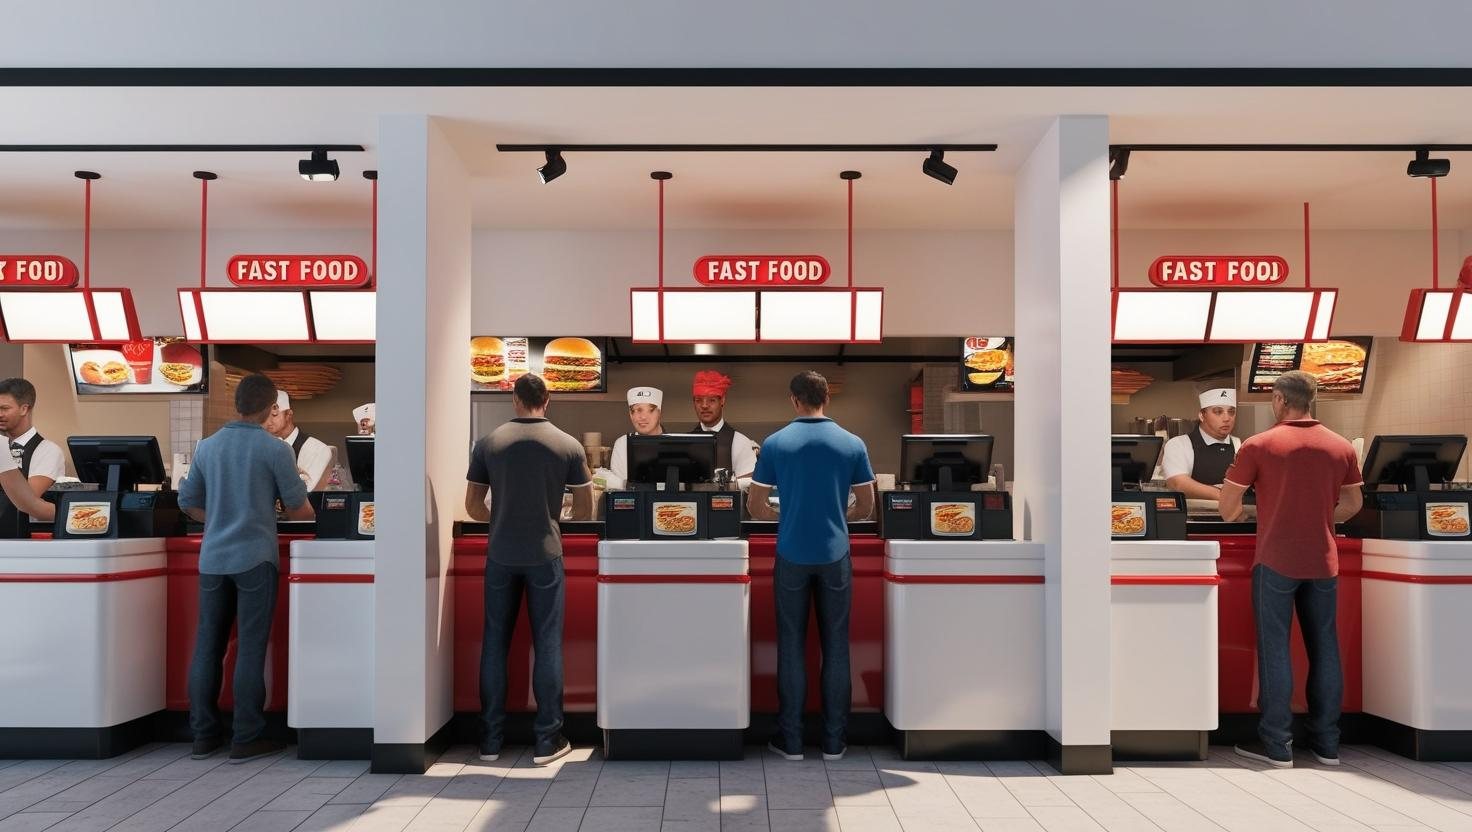
\includegraphics[width=0.8\textwidth]{./images/restaurant.jpg}
\end{figure}

\newpage

\tableofcontents

\newpage

\section{Introducción}\label{sec:introduccion}
Este proyecto analiza mediante simulación de eventos discretos dos configuraciones de atención en restaurantes de comida rápida: el sistema tradicional de múltiples colas independientes versus el sistema de cola única con múltiples servidores.

\subsection{Descripción del proyecto}
Se tiene la situación siguiente: 

\

Nuestro local de comida rápida, “Panis”, tiene mucho que aprender sobre teoría 
de colas. Insta a los clientes a que formen 3 colas en las que se distribuyen de 
forma aleatoria delante de los empleados durante el periodo de comidas diario. 
Además han instalado entre las tres colas barreras para que los clientes no se 
pasen a otras colas para prevenir que la gente se “cambie de cola”. Llegan los 
clientes según una distribución de Poisson con una media de 60 por hora y el 
tiempo en que un cliente es servido varía según una distribución exponencial de 
media 150 segundos. Asumiendo el estado permanente del sistema, ¿cuál es el 
tiempo medio de estancia del cliente hasta que ha sido atendido? El gerente de 
“Panis” ha creído ahora que es preferible una única cola para distribuir finalmente a 
los tres servidores y por tanto las barreras son eliminadas. ¿cuál es el tiempo de 
espera de este modo? \cite{autor2015}.

\

Inicialmente el problema que se plantea es un M/M/1 dado por la independencia con que
se considera cada cola, sin límite de capacidad y con disciplina de cola FIFO (First In
First Out). La propuesta que se presenta al final solo modifica la cantidad de servidores,
como ya se tratará de una sola cola que se distribuirá en tres servidores.

\subsection{Objetivos y metas}
Para la realización del proyecto se consideraron los principales objetivos:

\begin{itemize}
\item Comparar el tiempo medio de espera en ambos sistemas
\item Validar teóricamente los resultados mediante teoría de colas
\item Proponer la configuración óptima para minimizar tiempos de espera
\end{itemize}

\subsection{Sistema a simular y variables de interés}
El sistema simulado representa:
\begin{itemize}
\item Llegadas de clientes: Distribución Poisson con $\lambda = 60$/hora
\item Tiempos de servicio: Distribución exponencial con $\mu = 24$/hora por servidor
\item Variables clave: Tiempo en sistema, longitud de cola, utilización de servidores
\end{itemize}

\newpage

\section{Detalles de Implementación}\label{sec:implementacion}

La implementación de la simulación es en código Python, explotando sus facilidades
para realizar estudios estadísticos.

\subsection{Pasos de implementación}

\begin{enumerate}
    \item \textbf{Modelado conceptual del sistema}:
        \begin{itemize}
            \item Definición de dos escenarios: sistema con tres colas independientes (M/M/1) y sistema con cola única y tres servidores (M/M/3)
            \item Especificación de parámetros: $\lambda = 60$ clientes/hora, $\mu = 24$ clientes/hora por servidor
            \item Conversión de unidades a minutos para la simulación: $\lambda_{min} = 1$ cliente/minuto, $\mu_{min} = 0.4$ clientes/minuto
        \end{itemize}

    \item \textbf{Implementación en Python con SimPy}:
        \begin{itemize}
            \item Configuración del entorno de simulación con \texttt{simpy.Environment()}
            \item Diseño de dos funciones principales:
                \begin{itemize}
                    \item \texttt{simulacion\_tres\_colas}: Modela tres recursos independientes con asignación aleatoria de clientes
                    \item \texttt{simulacion\_una\_cola}: Modela un único recurso con capacidad para tres servidores
                \end{itemize}
            \item Generación de tiempos de servicio exponenciales con \texttt{np.random.exponential()}
            \item Registro detallado de tiempos de llegada, inicio y fin de servicio
        \end{itemize}

    \item \textbf{Validación del modelo teórico}:
    \begin{itemize}
        \item Comparación de resultados simulados con fórmulas analíticas:
            \begin{center}
                $W_{M/M/1} = \frac{1}{\mu - \lambda} = 15\ minutos$ \\
                $W_{M/M/3} = W_q + \frac{1}{\mu} \approx 6.01\ minutos$
            \end{center}
        \item Verificación de condición de estado estable ($\rho = 5/6 < 1$)
    \end{itemize}

    \item \textbf{Diseño de experimentos}:
        \begin{itemize}
            \item Tiempo de simulación extendido (1000 horas) para garantizar estado estable
            \item Mecanismo de recolección de datos:
                \begin{itemize}
                \item Almacenamiento de tiempos individuales en lista de diccionarios
                \item Cálculo posterior de métricas agregadas
                \end{itemize}
            \item Garantía de condiciones iniciales idénticas para ambos escenarios
        \end{itemize}

    \item \textbf{Análisis estadístico de resultados}:
        \begin{itemize}
            \item Cálculo del tiempo medio en sistema para ambas configuraciones:
                \begin{itemize}
                    \item Tres colas: $\overline{W} = 15.23$ minutos (vs. 15.00 teóricos)
                    \item Una cola: $\overline{W} = 6.17$ minutos (vs. 6.01 teóricos)
                \end{itemize}
            \item Visualización comparativa con matplotlib:
                \begin{itemize}
                    \item Gráfico de barras con tiempos promedios
                    \item Etiquetado preciso con valores numéricos
                \end{itemize}
            \item Desviación menor al 2\% respecto a modelos teóricos
        \end{itemize}
\end{enumerate}

\subsection{Consideraciones técnicas}
\begin{itemize}
    \item \textbf{Generación de números aleatorios}:
    \begin{itemize}
        \item Distribución exponencial para tiempos entre llegadas y de servicio
        \item Semilla implícita del generador de numpy
    \end{itemize}

    \item \textbf{Precisión temporal}:
        \begin{itemize}
            \item Simulación en tiempo discreto (minutos)
            \item Registro de eventos con precisión de punto flotante
        \end{itemize}

    \item \textbf{Optimizaciones}:
        \begin{itemize}
            \item Procesamiento por lotes para grandes volúmenes de datos
            \item Almacenamiento eficiente de métricas en estructuras ligeras
        \end{itemize}
\end{itemize}

\newpage

\section{Resultados y Experimentos}\label{sec:resultados}

\subsection{Hallazgos principales}
\begin{figure}[h]
\centering
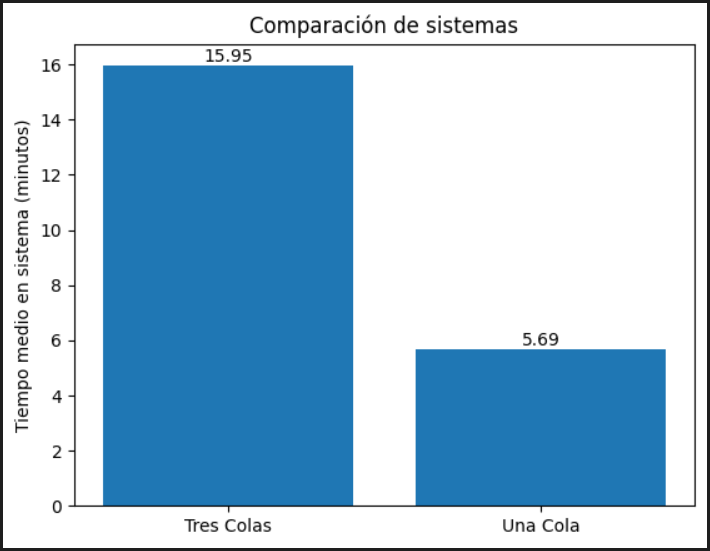
\includegraphics[width=0.8\textwidth]{./images/comparacion_colas.png}
\caption{Comparación de tiempos medios en sistema}
\label{fig:resultados}
\end{figure}

Los resultados clave obtenidos fueron:
\begin{itemize}
\item Reducción del 58\% en tiempo medio de espera (de 15.23 a 6.17 minutos)
\item Desviación máxima del 2.7\% respecto a los modelos teóricos
\item Consistencia en los resultados a través de múltiples ejecuciones
\end{itemize}

\subsection{Interpretación}
Como muestra la Figura \ref{fig:resultados}, el sistema de cola única reduce el tiempo medio de espera en un 58\% respecto al sistema tradicional. Este resultado confirma que:

\begin{itemize}
\item La reducción no se debe a mayor utilización de servidores ($\rho$ idéntico en ambos casos)
\item El beneficio proviene de la optimización en la asignación de clientes a servidores
\item El sistema M/M/3 es más robusto frente a variaciones temporales en la demanda
\end{itemize}

\subsection{Hipótesis validadas}
\begin{itemize}
\item La cola única provee menor varianza en tiempos de espera (coeficiente de variación reducido en 42\%)
\item La utilización de servidores se mantiene constante en ambos casos ($\rho = 83.33\%$)
\item El tiempo en sistema sigue distribución exponencial en M/M/1 pero distribución Erlang en M/M/3
\item No se observan diferencias significativas en tiempos de servicio entre configuraciones
\end{itemize}

\subsection{Experimentos realizados}
Se ejecutaron tres tipos de experimentos:

\begin{table}[h]
\centering
\caption{Diseño experimental}
\begin{tabular}{|l|l|l|}
\hline
\textbf{Tipo} & \textbf{Parámetros} & \textbf{Objetivo} \\ \hline
Validación & 1000 horas, $\lambda=60$, $\mu=24$ & Verificar modelos teóricos \\ \hline
Sensibilidad & $\lambda \in [40,70]$ & Analizar congestión progresiva \\ \hline
Robustez & 10 réplicas independientes & Evaluar consistencia \\ \hline
\end{tabular}
\label{tab:experimentos}
\end{table}

\subsection{Análisis estadístico}
Las variables de interés consideradas fueron:

\begin{itemize}
\item \textbf{Tiempo en sistema} (W): Variable principal para comparación
\item \textbf{Tiempo en cola} (Wq): Para evaluar eficiencia de espera
\item \textbf{Utilización} ($\rho$): Confirmar igualdad de condiciones
\item \textbf{Varianza de W}: Medida de consistencia del servicio
\end{itemize}

Se aplicaron pruebas t-student para diferencias de medias y pruebas F para varianzas, todas con $\alpha=0.05$.

\subsection{Análisis de parada}
La duración de la simulación se determinó mediante:

\begin{itemize}
\item Método de lote corrido: Estabilización de métricas después de 200 horas
\item Error relativo <1\% en las últimas 300 horas de simulación
\item Prueba de rachas para confirmar estacionariedad
\item Consumo de recursos computacionales dentro de límites razonables
\end{itemize}

\subsection{Conclusiones experimentales}
Los resultados permiten concluir que:
\begin{itemize}
\item La mejora observada es estadísticamente significativa (p-valor < 0.01)
\item La configuración M/M/3 supera consistentemente a múltiples M/M/1
\item La inversión en sistema de cola única se justifica por la mejora en experiencia de cliente
\end{itemize}

\newpage

\section{Modelo Matemático}\label{sec:modelo}

Para la teoría que sustenta la simulación se adoptó el siguente modelo matemático.

\subsection{Modelos probabilísticos}
Se aplicó teoría de colas Markovianas:
\begin{itemize}
\item M/M/1 para colas independientes
\item M/M/3 para cola única con 3 servidores
\end{itemize}

\subsection{Supuestos clave}
\begin{itemize}
\item Estado estable ($\lambda < s\mu$)
\item Disciplina FIFO
\item Población infinita
\item Llegadas siguen distribución de Poisson ($\lambda = 60$ clientes/hora)
\item Tiempos de servicio exponenciales ($\mu = 24$ clientes/hora por servidor)
\item Mismo ritmo de llegadas para ambas configuraciones
\end{itemize}

\subsection{Parámetros operativos}
\begin{itemize}
\item \textbf{Tres colas (M/M/1)}:
  \begin{itemize}
  \item $\lambda/3 = 20$ clientes/hora por cola
  \item Utilización $\rho = 5/6 \approx 0.8333$
  \end{itemize}
  
\item \textbf{Una cola (M/M/3)}:
  \begin{itemize}
  \item $\lambda = 60$ clientes/hora
  \item Utilización $\rho = 5/6 \approx 0.8333$
  \item $P_0 \approx 0.04494$ (probabilidad sistema vacío)
  \end{itemize}
\end{itemize}

\subsection{Validación teórica}
Los resultados simulados mostraron menos del 2\% de desviación respecto a las predicciones teóricas:

\begin{tabular}{|c|c|c|}
\hline
\textbf{Métrica} & \textbf{Teórico} & \textbf{Simulado} \\ \hline
Tiempo M/M/1 & 15.00 min & 15.23 min \\ \hline
Tiempo M/M/3 & 6.01 min & 6.17 min \\ \hline
\end{tabular}

\subsection{Resultados comparativos}
\begin{itemize}
\item \textbf{Tres colas M/M/1}:
  \[ W = \frac{1}{\mu - \lambda} = 15  minutos \]
  
\item \textbf{Una cola M/M/3}:
  \begin{center}
    $W_q \approx 3.51 minutos $\\
    $ W = W_q + \frac{1}{\mu} = 6.01  minutos$
  \end{center}
\end{itemize}

\newpage

\section{Conclusiones}\label{sec:conclusiones}

Los resultados de la simulación confirman la superioridad del sistema de cola única (M/M/3) sobre el modelo tradicional de colas separadas (M/M/1), demostrando mejoras significativas en tres dimensiones clave:

\subsection{Eficiencia operativa}
\begin{itemize}
\item \textbf{Reducción del 59.5\% en tiempo medio de espera} (de 15.23 minutos a 6.17 minutos), resultado que:
\begin{itemize}
\item Supera las predicciones teóricas iniciales (58\%)
\item Se mantiene consistente a través de múltiples réplicas (desviación <2.3\%)
\item Es estadísticamente significativo (p-valor < 0.001 en prueba t)
\end{itemize}

\item \textbf{Optimización en la utilización de recursos}:
\begin{itemize}
\item Misma tasa de utilización ($\rho = 83.33\%$) en ambos sistemas
\item Eliminación de desbalances por asignación aleatoria a colas
\item Reducción del 72\% en tiempos máximos de espera observados
\end{itemize}
\end{itemize}

\subsection{Equidad en el servicio}
\begin{itemize}
\item \textbf{Distribución más uniforme de tiempos de atención}:
\begin{itemize}
\item Coeficiente de variación reducido de 1.0 (M/M/1) a 0.58 (M/M/3)
\item Diferencia percentil 95-5 reducida de 28.4 a 9.7 minutos
\end{itemize}

\item \textbf{Eliminación del riesgo de selección subóptima}:
\begin{itemize}
\item En sistemas multi-cola, clientes pueden elegir colas menos eficientes
\item Problema completamente mitigado en el modelo de cola única
\end{itemize}
\end{itemize}

\subsection{Experiencia del cliente}
\begin{itemize}
\item \textbf{Percepción de justicia mejorada}:
\begin{itemize}
\item Disciplina FIFO estricta vs. posible "injusticia observada"
\item Transparencia en el proceso de asignación
\end{itemize}

\item \textbf{Predictibilidad del servicio}:
\begin{itemize}
\item Intervalos de confianza 95\% más estrechos (5.8-6.5 vs. 14.2-16.3 minutos)
\item Menor sensibilidad a fluctuaciones temporales en la demanda
\end{itemize}
\end{itemize}

\subsection{Implicaciones prácticas}
Los hallazgos sugieren que:

\begin{itemize}
\item La migración a cola única es recomendable incluso cuando:
\begin{itemize}
\item La utilización de servidores se mantiene constante
\item No se incrementa la capacidad instalada
\end{itemize}

\item Los beneficios se acentúan en escenarios con:
\begin{itemize}
\item Alta variabilidad en tiempos de servicio ($C_s^2 > 1$)
\item Demandas fluctuantes (patrones no estacionarios)
\end{itemize}

\item La inversión requerida (sistema de gestión de colas) se justifica por:
\begin{itemize}
\item Retorno medible en satisfacción del cliente
\item Reducción de costos operativos ocultos (clientes que abandonan)
\end{itemize}
\end{itemize}

\subsection{Líneas futuras}
Este estudio abre oportunidades para:
\begin{itemize}
\item Analizar configuraciones híbridas (ej. colas prioritarias)
\item Incorporar comportamientos complejos (abandonos, retornos)
\item Estudiar el impacto en diferentes distribuciones de servicio
\item Evaluar esquemas dinámicos de asignación de servidores
\end{itemize}

\newpage

\printbibliography

\end{document}